\documentclass[10pt,a4paper]{article}
\usepackage[margin=2.2cm]{geometry}
\usepackage{fontspec}
\usepackage{kotex}
\setmainfont{Apple SD Gothic Neo}
\setsansfont{Apple SD Gothic Neo}
\usepackage{amsmath,amssymb}
\usepackage{graphicx}
\usepackage{booktabs}
\usepackage{caption}
\usepackage[dvipsnames]{xcolor}
\usepackage[colorlinks=true,linkcolor=MidnightBlue,citecolor=MidnightBlue,
            urlcolor=MidnightBlue]{hyperref}
\usepackage{titlesec}
\titleformat{\section}{\large\bfseries}{\thesection}{0.6em}{}
\titleformat{\subsection}{\normalsize\bfseries}{\thesubsection}{0.5em}{}
\captionsetup{font=small,labelfont=bf}
\setlength{\parskip}{0.35em}
\setlength{\parindent}{0pt}

\usepackage{mdframed}
\newmdenv[linewidth=0.4pt,linecolor=gray!60,backgroundcolor=gray!5,
          innertopmargin=6pt,innerbottommargin=6pt,skipabove=8pt,skipbelow=8pt]{claimbox}
\newcommand{\claim}[2]{\begin{claimbox}\textbf{주장.} #1\par\smallskip
  \textcolor{gray!70}{\textbf{반증 조건.} #2}\end{claimbox}}

\title{\bfseries 다섯 문을 다 닫았다\\[2pt]
\large 기제 후보 다섯 중 하나만 부분 성공했고 --- 그래서 ``왜''를 접는다}
\author{월드모델 실험실 · 노트 763 · 764 · 765}
\date{2026-08-07}
\begin{document}\maketitle

\section{한 줄}

논문 $147 \sim 149$ 가 \textbf{장의 전국 시간축이 판을 해친다}는 것을 확정하고 기제
후보를 하나씩 지웠다. 여기서 마지막 후보(\textbf{감쇠})를 지웠다 --- 감쇠량
$\leftrightarrow$ 신호 몫 스피어만 $\mathbf{+0.009}$($p{=}0.979$).

\textbf{후보 다섯 중 하나만 부분 성공했다}(공변량 이동 · $59\%$). 사전등록 규칙이
\emph{``후보가 다 떨어지면 왜 를 접고 무엇을 대신 쓰나 로 옮긴다''}를 적어 뒀고,
\textbf{그것을 따른다.}

\section{먼저 배선을 읽었고, 그것이 가설 둘을 죽였다}

논문 $149$ 가 다음 실험으로 \emph{``웹툰 · 도서를 뺀 판에서 다시 잰다''}를 등록했다.
\textbf{그것이 공짜인지 보려고 채점 코드를 읽었다.} 두 사실이 나왔다.

\begin{center}
\begin{tabular}{ll}
\toprule
\textbf{① 공동 적합} & \texttt{evaluate} 가 \textbf{모형 하나}를 전 도메인 학습 행으로
적합하고 도메인마다 채점한다 \\
\textbf{② 순위 채점} & \texttt{\_score\_one} 이 \textbf{그 도메인 유보 행 안에서}
\texttt{spearman(예측, 라벨)} 을 낸다 \\
\bottomrule
\end{tabular}
\end{center}

\claim{\textbf{② 때문에 가설 둘이 재기 전에 죽었다.} 나는 논문 $149$ 에서 \emph{``웹툰 ·
도서는 둘 다 연재물이고 라벨이 누적형이라 시점 상태와 안 맞는다''}를 적었다.
\textbf{그것은 라벨 \emph{수준}에 관한 가설이고, 유보 안 순위 채점에서는 수준이 무관하다.}
같은 이유로 ``유보 라벨이 작아서'' 류의 설명이 전부 죽는다. \textbf{규율: 기제를
세우기 전에 채점 규칙을 읽는다} --- 노트 $749$(\emph{``이상값은 설명 전에
재현한다''})의 짝이다.}
{읽어서 죽인 것이 옳은지는 ``수준이 순위에 전혀 안 새는가''에 달렸다. 라벨 수준이
바뀌면 \emph{순위 구조}도 같이 바뀔 수 있으므로(예: 상한에 눌리는 라벨) 완전히 무관하다고
말할 수는 없다. \textbf{그러나 그 경우 검사 대상은 ``수준''이 아니라 ``순위 압축''이고,
가설을 그렇게 다시 적어야 한다.}}

\claim{\textbf{① 은 지금까지의 도메인별 수치를 읽는 법을 바꾼다.} 모형이 공동 적합이므로
어떤 도메인의 신호 몫은 \textbf{그 도메인 자료만의 성질이 아니다} --- \textbf{다른
도메인이 모형에 준 관계가 그 도메인에 맞나}를 같이 담는다. 그리고 \textbf{한 도메인을
학습에서 빼면 다른 도메인 점수도 바뀐다} --- 등록된 실험은 공짜가 아니었다.}
{그래서 ``국소적이다''를 재적합으로 확정하려면 도메인마다 빼고 다시 적합해야 하고,
그때 \textbf{빠진 도메인 때문에 좋아진 것과 그 도메인이 어려워서 나빴던 것}이 다시
섞인다. \textbf{깔끔한 식별이 없다} --- 그것이 이 실험을 안 돌린 이유이기도 하다.}

\subsection*{공짜로 답한 것}

노트 $762$ 의 도메인별 신호 몫과 유보 가중으로 \textbf{웹툰($650$) · 도서($163$)를
채점에서만 뺀 신호 몫}을 계산했다 --- \textbf{$+0.0032$}(가중 합 $8.2745 \div 2{,}556$).
\textbf{문턱($0.0045$) 안이고 양수다.} \textbf{다만 재적합이 아니라 재가중이다} ---
모형은 여전히 그 둘을 학습에 썼다.

\begin{figure}[t]\centering
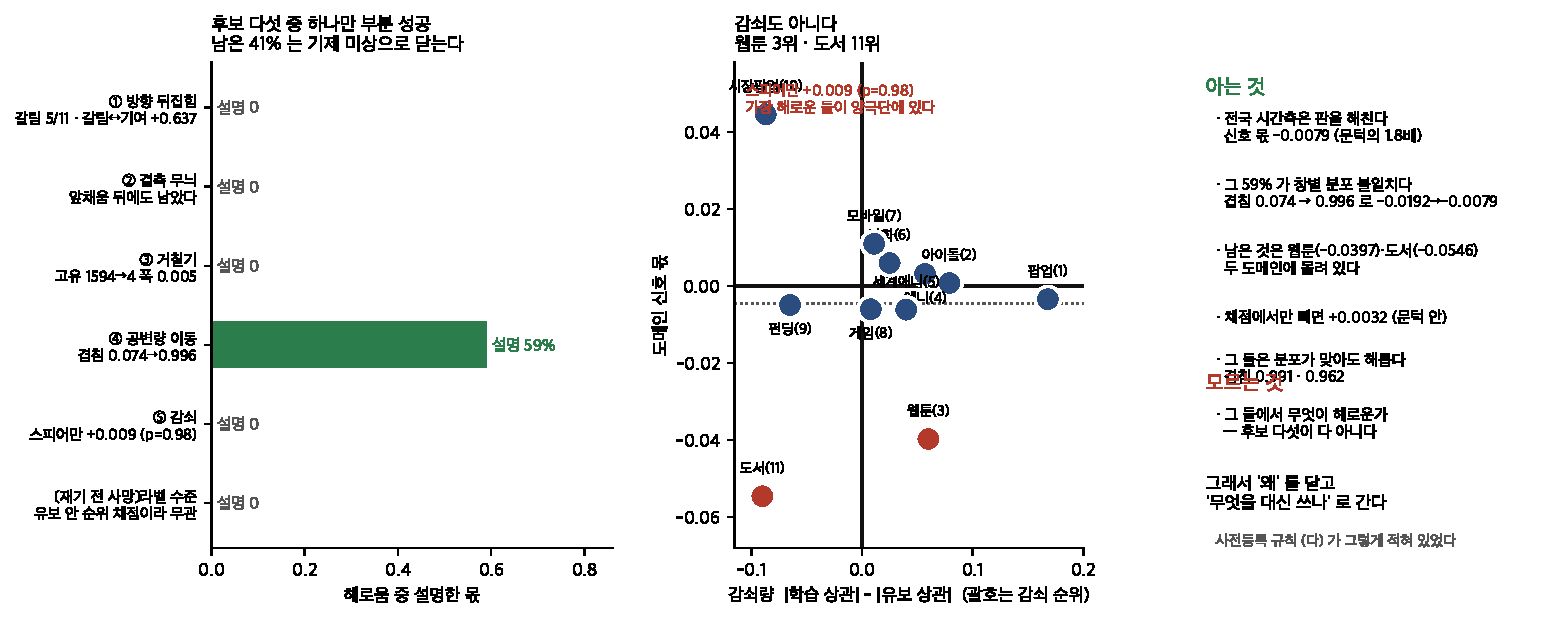
\includegraphics[width=0.99\textwidth]{figs/fivedoors.pdf}
\caption{왼쪽: \textbf{후보 다섯 중 하나만 부분 성공}. 가운데: \textbf{감쇠는
무관하다} --- 가장 해로운 둘이 감쇠 순위의 양극단에 있다. 오른쪽: \textbf{아는 것과
모르는 것}을 갈라 적었다.}
\end{figure}

\section{마지막 후보 --- 감쇠도 아니다}

논문 $149$ 가 실마리를 남겼다: 가장 해로운 둘에서 학습 상관 $0.08$ 이 유보에서
$0.02$ 로 \textbf{감쇠}한다. 공동 적합이므로 \emph{``모형이 배운 관계가 그 도메인
유보에서 안 남으면 과신해서 틀린다''}가 자연스러운 가설이다.

\begin{center}
\begin{tabular}{lrl}
\toprule
\textbf{감쇠량}($|$학습$| - |$유보$|$) $\leftrightarrow$ \textbf{신호 몫} 스피어만
& $\mathbf{+0.009}$ & $p = 0.979$ \\
웹툰 감쇠 순위 & $3 / 11$ & 가장 해로운 도메인 \\
도서 감쇠 순위 & $\mathbf{11 / 11}$ & \textbf{가장 감쇠가 적다} \\
학습 $|$상관$|$ 중앙값 & $0.051$ & 약하다 \\
\bottomrule
\end{tabular}
\end{center}

\textbf{완전히 무관하고, 가장 해로운 둘이 감쇠 순위의 양극단에 있다.} 사전등록 규칙
(다) 발동.

\subsection*{틀림 조건이 같이 발동했고 그것도 배움이다}

\emph{``창 안 백분위 축의 상관이 앞과 거의 같으면 이 실험이 새 정보를 안 준다''}를
미리 적었고 \textbf{중앙 절대차가 $0.000$ 이다} --- 완전히 같다. \textbf{이유가 뒤늦게
자명하다}: 학습 상관은 \textbf{학습 행 안에서만} 계산하고, 전 구간 백분위든 창 안
백분위든 \textbf{학습 행끼리의 상대 순위는 같다.}

\claim{\textbf{순위 지표로는 안 보이는 개선이 있다.} 창 안 백분위로 바꾸니 판 신호
몫이 $-0.0192 \to -0.0079$($59\%$ 개선)인데 \textbf{도메인 안 축$\leftrightarrow$라벨
스피어만은 소수 셋째 자리까지 그대로}다. \textbf{즉 상관이 안 변해도 분포를 맞추면
트리의 분할점이 유보에서 유효해진다} --- \textbf{축을 상관으로만 평가하면 이 이득을
못 본다.}}
{개선이 분포 맞춤 때문이 아니라 \textbf{창 안 순위 매김이 만든 다른 무엇} 때문일 수도
있다. 가르려면 분포는 맞추되 순위를 보존하는 변환이 필요하고, 논문 $149$ 에서도
같은 한계를 적었다 --- \textbf{두 번 같은 미측정이 남아 있다.}}

\section{그래서 ``왜''를 닫는다}

\begin{center}
\begin{tabular}{lll}
\toprule
후보 & 결과 & 근거 \\
\midrule
① 방향 뒤집힘 & \textbf{아니다} & 갈림 $5/11$ · 가장 해로운 둘 안 갈림 · 갈림$\leftrightarrow$기여 $+0.637$ \\
② 결측 무늬 & \textbf{아니다} & 덮음 $0.53$ 은 공짜 · 앞채움 뒤에도 남았다 \\
③ 거칠기 & \textbf{아니다} & 고유 $1{,}594 \to 4$ 에서 폭 $0.005$(문턱 $0.010$ 미달) \\
\textbf{④ 공변량 이동} & \textbf{$59\%$} & 겹침 $0.074 \to 0.996$ 으로 $-0.0192 \to -0.0079$ \\
⑤ 감쇠 & \textbf{아니다} & 스피어만 $+0.009$ \\
\midrule
〔재기 전 사망〕라벨 수준 & --- & 유보 안 순위 채점이라 무관 \\
\bottomrule
\end{tabular}
\end{center}

\claim{\textbf{아는 것과 모르는 것을 갈라 적고 닫는다.} \textbf{아는 것} --- 전국 시간축은
판을 해친다(신호 몫 $-0.0079$ · 문턱의 $1.8$배 음수) · 해로움의 $59\%$ 가 창별 분포
불일치다 · 나머지는 웹툰($-0.0397$) · 도서($-0.0546$) 두 도메인에 몰려 있다(채점에서만
빼면 $+0.0032$) · \textbf{그 둘은 분포가 맞아도 해롭다}(겹침 $0.991 \cdot 0.962$).
\textbf{모르는 것} --- 그 둘에서 무엇이 해로운가. \textbf{후보 다섯이 다 아니다.}}
{여섯째 후보가 있을 수 있다 --- 예컨대 \textbf{순위 압축}(라벨이 상한에 눌려 순위가
뭉치는 것)이나 \textbf{공동 적합의 상호작용}(다른 도메인이 준 관계가 그 둘에만 안
맞는 것)이다. \textbf{후자는 도메인별 재적합으로 재야 하고 위에 적은 식별 문제가
걸린다.} \textbf{그래서 ``닫는다''는 ``없다''가 아니라 ``이 사이클에서 더 파지
않는다''다.}}

\subsection*{닫는 것이 규율인 이유}

노트 $749$ 가 \emph{``재현 안 된 이상값을 두 사이클 동안 설명하려 했다''}를 적었다.
\textbf{이번에는 반대 위험이 있다} --- 다섯 문을 닫고도 여섯째를 찾아 계속 파는 것.
사전등록 규칙 (다)가 그 자리에서 \textbf{멈추라}고 적혀 있었고, \textbf{규칙을 결과
보기 전에 적었기 때문에 그것을 따를 수 있다.}

\begin{center}
\textbf{T2 는 이제 ``왜''를 접고 ``무엇을 대신 쓰나''로 간다.}\\
다음: \textbf{IP 에 지역을 붙일 수 있나} --- 읽기 전용으로 센다.
\end{center}

\end{document}
